\documentclass[11pt,a4paper,openany]{book}

\makeatletter\def\input@path{{../_shared/}}\makeatother
\usepackage{course}

\begin{document}
\raggedbottom

\coursetitle{Algorithms I}{BA4}{2025--2026}

\tableofcontents
\clearpage

These notes cover the core algorithmique techniques of the BA4 Algorithms I course:
asymptotic analysis, sorting, divide-and-conquer, heaps, binary search trees, and
graph algorithms (max flow, matchings).

% =========================================================
\chapter{Algorithms Fundamentals}
% =========================================================

\section{Definition of an Algorithm}
\begin{defnbox}
An \textbf{algorithm} is a well-defined computational procedure that takes some value (or
set of values) as \emph{input} and produces some value (or set of values) as \emph{output}
in a finite number of steps.
\end{defnbox}

We analyse algorithms along two axes:
\begin{itemize}
  \item \textbf{Correctness} — does it always produce the right answer?
  \item \textbf{Efficiency} — how many resources (time, space) does it consume?
\end{itemize}

% ---------------------------------------------------------
\section{Asymptotic Complexity}
% ---------------------------------------------------------

\begin{defnbox}[title=Asymptotic notations]
Let $f, g : \mathbb{N} \to \mathbb{R}^+$.
\begin{itemize}
  \item $f \in O(g)$ \textbf{(upper bound)}: $\exists\, c, n_0 > 0$ s.t.\ $f(n) \leq c\,g(n)$ for all $n \geq n_0$
  \item $f \in \Omega(g)$ \textbf{(lower bound)}: $\exists\, c, n_0 > 0$ s.t.\ $f(n) \geq c\,g(n)$ for all $n \geq n_0$
  \item $f \in \Theta(g)$ \textbf{(tight bound)}: $f \in O(g)$ and $f \in \Omega(g)$
  \item $f \in o(g)$ \textbf{(strict upper)}: $\lim_{n\to\infty} f(n)/g(n) = 0 or also f(n) < g(n)$
  \item $f \in \omega(g)$ \textbf{(strict lower)}: $\lim_{n\to\infty} f(n)/g(n) = \infty or also f(n) > g(n)$
\end{itemize}
\end{defnbox}

\begin{propbox}[title=Common growth rates (slowest to fastest)]
\[
  O(1) \subset O(\log n) \subset O(n) \subset O(n\log n) \subset O(n^2)
  \subset O(n^3) \subset O(2^n) \subset O(n!)
\]
\end{propbox}

\begin{rembox}
For the \textbf{Master Theorem}: given $T(n) = a\,T(n/b) + f(n)$ with $a \geq 1$, $b > 1$:
\begin{itemize}
  \item if $f(n) = O(n^{\log_b a - \eps})$ then $T(n) = \Theta(n^{\log_b a})$
  \item if $f(n) = \Theta(n^{\log_b a})$ then $T(n) = \Theta(n^{\log_b a} \log n)$
  \item if $f(n) = \Omega(n^{\log_b a + \eps})$ then $T(n) = \Theta(f(n))$
\end{itemize}
\end{rembox}










% ---------------------------------------------------------
\chapter{Sorting Algorithms}
% ---------------------------------------------------------

\section{Insertion Sort}

\begin{propbox}[title=Complexity]
Time: $\Theta(n^2)$ worst/average, $\Theta(n)$ best (already sorted). \quad Space: $O(1)$ in-place.
\end{propbox}

\begin{lstlisting}[language=Python]
def insertion_sort(A):
    for j in range(1, len(A)):
        key = A[j]
        i = j - 1
        while i >= 0 and A[i] > key:
            A[i + 1] = A[i]
            i -= 1
        A[i + 1] = key
\end{lstlisting}

\begin{lstlisting}
Insertion-Sort(A, n)
    for j = 2 to n
        key = A[j]
        // Insert A[j] into the sorted sequence A[1...j - 1].
        i = j - 1
        while i > 0 and A[i] > key
            A[i + 1] = A[i]
            i = i - 1
        A[i + 1] = key
\end{lstlisting}

\textbf{Loop invariant:} at the start of each iteration, \texttt{A[0..j-1]} is sorted. \\
\textbf{Concept and objective:} Sort an array








\vspace{2cm}





% ---------------------------------------------------------
\section{Divide and Conquer principles}
% ---------------------------------------------------------

\begin{defnbox}[title=Paradigm]
\textbf{Divide} the problem into subproblems, \textbf{conquer} each recursively, then
\textbf{combine} the results.
\end{defnbox}










\vspace{2cm}









\section{Merge Sort}

\begin{propbox}[title=Complexity]
Time: $\Theta(n \log n)$ in all cases. \quad Space: $O(n)$ auxiliary.
\end{propbox}

\begin{lstlisting}[language=Python]
def merge_sort(A, p, r):
    if p < r:
        q = (p + r) // 2
        merge_sort(A, p, q)
        merge_sort(A, q + 1, r)
        merge(A, p, q, r)   # merge two sorted halves
\end{lstlisting}

\begin{lstlisting}
MERGE-SORT(A, p, r)
    if p < r                // check for base case
        q = rounddown((p + r)/2)     // divide
        MERGE-SORT(A, p, q) // conquer
        MERGE-SORT(A, q + 1, r) // conquer
        MERGE(A, p, q, r)   // combine

MERGE(A,p,q,r)
	n1 = q-p+1
	n2 = r-q
	let L[1...n1 + 1] and R[1 ... n2+1] be new arrays
	for i = 1 to n1
		L[i] = A[p+i-1]
	for j = 1 to n2
		R[j] = A[q+j]
	L[,1+1] = 8
	R[n2+1] = 8
	i = 1
	j = 1
	for k = p to r
		if L[i] <= R[j]
			A[k] = L[i]
			i = i + 1
		else A[k] = R[j]
			j = j + 1
\end{lstlisting}

\textbf{Recurrence:} $T(n) = 2\,T(n/2) + \Theta(n)$ $\Rightarrow$ $T(n) = \Theta(n \log n)$ by Master Theorem (case 2).
//
\textbf{Concept and objective:} Sort an array















\vspace{2cm}







\section{Master theorem}

\begin{defnbox}[title=Theorem (Master Theorem)]
Let $a \geq 1$ and $b > 1$ be constants, let $T(n)$ be defined on the nonnegative integers by the recurrence
\[
T(n)=aT(n/b)+f(n).
\]

Then, $T(n)$ has the following asymptotic bounds:

\begin{itemize}
    \item If $f(n)=O\!\left(n^{\log_b a-\epsilon}\right)$ for some constant $\epsilon>0$, then
    \[
    T(n)=\Theta\!\left(n^{\log_b a}\right).
    \]

    \item If $f(n)=\Theta\!\left(n^{\log_b a}\right)$, then
    \[
    T(n)=\Theta\!\left(n^{\log_b a}\log n\right).
    \]

    \item If $f(n)=\Omega\!\left(n^{\log_b a+\epsilon}\right)$ for some constant $\epsilon>0$, and if
    \[
    a\cdot f(n/b)\leq c\cdot f(n)
    \]
    for some constant $c<1$ and all sufficiently large $n$, then
    \[
    T(n)=\Theta\!\left(f(n)\right).
    \]
\end{itemize}
\end{defnbox}







\vspace{2cm}





% ---------------------------------------------------------
\chapter{Maximum Subarray, Matrix Multiplication and Strassen ect}
% ---------------------------------------------------------

\section{Maximum Subarray optimized}

Find indices $i \leq j$ maximising $\sum_{k=i}^{j} A[k]$.

\begin{propbox}[title=Complexity]
$T(n) = 2\,T(n/2) + \Theta(n)$ $\Rightarrow$ $\Theta(n \log n)$.
(Kadane's linear algorithm also exists: $\Theta(n)$.)
\end{propbox}

\begin{lstlisting}
FIND-MAXIMUM-SUBARRAY(A, low, high):
    if high == low: return (low, high, A[low])
    mid = (low + high) / 2
    left  = FIND-MAXIMUM-SUBARRAY(A, low, mid)
    right = FIND-MAXIMUM-SUBARRAY(A, mid+1, high)
    cross = FIND-MAX-CROSSING(A, low, mid, high)

    if left-sum >= right-sum and left-sum >= cross-sum
    return (left-low, left-high, left-sum)
    elseif right-sum >= left-sum and right-sum >= cross-sum
        return (right-low, right-high, right-sum)
    else
        return (cross-low, cross-high, cross-sum)
\end{lstlisting}

\begin{lstlisting}
FIND-MAX-CROSSING(A, low, mid, high)

  // Find a maximum subarray of the form A[i .. mid].
  left-sum = -8
  sum = 0
  for i = mid downto low
      sum = sum + A[i]
      if sum > left-sum
          left-sum = sum
          max-left = i

  // Find a maximum subarray of the form A[mid + 1 .. j].
  right-sum = -8
  sum = 0
  for j = mid + 1 to high
      sum = sum + A[j]
      if sum > right-sum
          right-sum = sum
          max-right = j

  // Return the indices and the sum of the two subarrays.
  return (max-left, max-right, left-sum + right-sum)
\end{lstlisting}
//
\textbf{Concept et objectif :}

L'algorithme \texttt{FIND-MAXIMUM-SUBARRAY} utilise la méthode du \textit{divide and conquer} (diviser pour régner).  
Son objectif est de trouver la sous-partie continue d'un tableau dont la somme des éléments est maximale, le
sous-enesemble de nombres qui font que leur somme est maximale. 

Le principe est simple :
\begin{itemize}
    \item le tableau est séparé en deux parties,
    \item l'algorithme cherche récursivement la meilleure sous-partie à gauche,
    \item puis la meilleure à droite,
    \item et enfin la meilleure sous-partie qui traverse le milieu.
\end{itemize}

Parmi ces trois possibilités, il retourne celle ayant la plus grande somme.









\vspace{2cm}


\section{Maximum Subarray BRUTE FORCE}


\begin{lstlisting}
MAXIMUM-SUBARRAY-SLOW(A[1..n]):

    B.val <- -8
    B.i <- 1
    B.j <- n

    for i <- 1 to n
        tmp <- 0

        for j <- i to n
            tmp <- tmp + A[j]

            if tmp > B.val
                B.val <- tmp
                B.i <- i
                B.j <- j

    return (B.i, B.j, B.val)
\end{lstlisting}

\textbf{Running time:}

\[
\Theta(n^2)
\]

\textbf{Space usage:}

\[
\Theta(n)
\]

(\(\Theta(n)\) for input + \(\Theta(1)\) extra)



\vspace{2cm}













\section{Matrix Multiplication naive}

Standard $O(n^3)$ triple loop, or the recursive divide-and-conquer that splits each
$n \times n$ matrix into four $n/2 \times n/2$ blocks: $T(n) = 8\,T(n/2) + \Theta(n^2)$,
giving the same $\Theta(n^3)$ by Master Theorem (case 1).


\begin{lstlisting}
SQUARE-MAT-MULT(A, B, n)
    let C be a new n x n matrix

    for i = 1 to n
        for j = 1 to n
            c_{ij} = 0
            for k = 1 to n
                c_{ij} = c_{ij} + a_{ik} * b_{kj}

    return C
\end{lstlisting}

\textbf{Goal:} Perform Matrix multiplication \\
\textbf{Time complexity:} $O(n^3)$ \\
\textbf{Space:} $O(n^2)$



\vspace{2cm}


\section{REC-MAT-MULT - other naive matrix multiplication - divide and conquer logic}

\begin{lstlisting}
REC-MAT-MULT(A, B, n)
    let C be a new n x n matrix

    if n == 1
        c11 = a11 * b11

    else
        partition A, B, and C into n/2 x n/2 submatrices

        C11 = REC-MAT-MULT(A11, B11, n/2) + REC-MAT-MULT(A12, B21, n/2)
        C12 = REC-MAT-MULT(A11, B12, n/2) + REC-MAT-MULT(A12, B22, n/2)
        C21 = REC-MAT-MULT(A21, B11, n/2) + REC-MAT-MULT(A22, B21, n/2)
        C22 = REC-MAT-MULT(A21, B12, n/2) + REC-MAT-MULT(A22, B22, n/2)

    return C
\end{lstlisting}

\textbf{Goal:} Perform matrix multiplication but here using divide and conquer logic\\
\textbf{Time complexity:} $O(n^3)$ \\
\textbf{Space:} $O(n^2)$








\vspace{2cm}






\section{Strassen's algorithm - better matrix multiplication}
\begin{propbox}[title=Complexity]
$T(n) = 7\,T(n/2) + \Theta(n^2)$ $\Rightarrow$ $\Theta(n^{\log_2 7}) \approx \Theta(n^{2.807})$.
\end{propbox}

Key idea: compute only 7 products of submatrices (instead of 8) using the following
auxiliary matrices $M_1, \ldots, M_7$, each a linear combination of blocks of $A$ and $B$:
\[
  M_1 = (A_{11}+A_{22})(B_{11}+B_{22}), \quad
  M_2 = (A_{21}+A_{22})B_{11}, \quad \ldots
\]
Then reconstruct $C_{11}, C_{12}, C_{21}, C_{22}$ from $M_1$--$M_7$.



\begin{lstlisting}
STRASSEN-MAT-MULT(A, B, n)
    let C be a new n * n matrix
    if n == 1
        C11 = A11 * B11
    else
        partition A, B, and C into n/2 x n/2 submatrices

        M1 = (A11 + A22) * (B11 + B22)
        M2 = (A21 + A22) * B11
        M3 = A11 * (B12 - B22)
        M4 = A22 * (B21 - B11)
        M5 = (A11 + A12) * B22
        M6 = (A21 - A11) * (B11 + B12)
        M7 = (A12 - A22) * (B21 + B22)

        C11 = M1 + M4 - M5 + M7
        C12 = M3 + M5
        C21 = M2 + M4
        C22 = M1 - M2 + M3 + M6

    return C
\end{lstlisting}

\textbf{Goal:} Perform matrix multiplication more efficiently than the classical method \\
\textbf{Time complexity:} $O(n^{\log_2 7})$ \\
\textbf{Space:} $O(n^2)$ \\
\textbf{Idea:} Reduce the number of recursive multiplications from 8 to 7 by using clever linear combinations of submatrices.






\vspace{2cm}






\subsection{Karatsuba Multiplication}

Multiply two $n$-digit integers (en base b n'importe laquelle) faster than the naive $O(n^2)$ schoolbook method.
Pourquoi est-ce qu'on en parle maintenant ? Parce que tout simplement
ça va utiliser un peu la même logique que Strassen's algorithm parce que on va séparer
en différents calculs qui vont nous permettre de résuire au final le nombre de multiplicationsà réaliser.

Split: $x = x_H b^{n/2} + x_L$, $y = y_H b^{n/2} + y_L$.

Compute only 3 multiplications:
\[
  p_1 = x_H \cdot y_H, \quad
  p_2 = x_L \cdot y_L, \quad
  p_3 = (x_H + x_L)(y_H + y_L)
\]
then $x \cdot y = p_1 b^n + (p_3 - p_1 - p_2)\,b^{n/2} + p_2$.

\begin{propbox}[title=Complexity]
$T(n) = 3\,T(n/2) + \Theta(n)$ $\Rightarrow$ $\Theta(n^{\log_2 3}) \approx \Theta(n^{1.585})$.
\end{propbox}

Ceci n'estr  pas un pseudocode pseudocodesque mais ça explique bien le principe
de l'algo: 

\begin{lstlisting}
KARATSUBA-MULT(x, y, n)
    if n == 1
        return x * y

    else
        split x into xH, xL
        split y into yH, yL

        p1 = KARATSUBA-MULT(xH, yH, n/2)
        p2 = KARATSUBA-MULT(xL, yL, n/2)
        p3 = KARATSUBA-MULT(xH + xL, yH + yL, n/2)

        return p1 * b^n + (p3 - p1 - p2) * b^(n/2) + p2
\end{lstlisting}

\textbf{Goal:} Perform multiplication faster than the naive method \\
\textbf{Time complexity:} $O(n^{\log_2 3})$ \\

\textbf{Space:} $O(1)$






\vspace{2cm}








% ---------------------------------------------------------
\chapter{Heap data structure}
% ---------------------------------------------------------

\begin{defnbox}[title=Heap]

Un \textbf{heap} (ou tas) est une structure de données sous forme d’arbre binaire presque complet, utilisée pour gérer efficacement des priorités.

COMMENT ON LE STOCKE DANS UN COMPUTER ?????????? \\
Il est généralement stocké sous forme de tableau :
\[
\begin{aligned}
\text{LEFT}(i) &= 2i \\
\text{RIGHT}(i) &= 2i + 1 \\
\text{PARENT}(i) &= \left\lfloor \frac{i}{2} \right\rfloor
\end{aligned}
\]
Cette structure est très utilisée pour les files de priorité et l’algorithme de tri \textit{heapsort}.
\end{defnbox}


\begin{defnbox}[title=Max-heap property]
A \textbf{max-heap} is a nearly complete binary tree where every node satisfies
$A[\text{parent}(i)] \geq A[i]$.
\end{defnbox}

\begin{defnbox}[title=Min-heap property]
A \textbf{min-heap} is a nearly complete binary tree where every node satisfies
$A[\text{parent}(i)] \leq A[i]$.
\end{defnbox}







\begin{defnbox}[title=Root]
The \textbf{root} is the top node of the heap. In array representation, it is at index 1.  
In a max-heap, it contains the largest element.
\end{defnbox}

\begin{defnbox}[title=Leaf]
A \textbf{leaf} is a node with no children.  
Leaves are located at the bottom level of the heap.
\end{defnbox}

\begin{defnbox}[title=Height]
The \textbf{height} of a heap is the number of edges on the longest path from the root to a leaf.  
A heap of size $n$ has height $\Theta(\log n)$.
\end{defnbox}

\begin{defnbox}[title=Height of a node]
Height of node is the number of edges on a longest simple path from the node
down to a leaf. (logiquement ça ne peut pas être plus grand que la height du tree en entier)
\end{defnbox}

\begin{defnbox}[title=Shape property]
A heap is a \textbf{complete binary tree}: all levels are full except possibly the last, which is filled from left to right.
\end{defnbox}





\vspace{2cm}




\section{MAX-HEAPIFY}

Ce qu'on veut maintenant c'est un algorithm capable de prendre un heap et d'en 
faire un max heap donc on utilise MAX HEAPIFY
\textbf{Algorithme :}
\begin{itemize}
    \item Comparer $A[i]$, $A[\mathrm{LEFT}(i)]$ et $A[\mathrm{RIGHT}(i)]$.
    
    \item Si nécessaire, échanger $A[i]$ avec le plus grand de ses deux enfants afin de préserver la propriété de tas (heap).
    
    \item Continuer ce processus de comparaison et d'échange vers le bas du tas jusqu'à ce que le sous-arbre enraciné en $i$ soit un max-heap.
\end{itemize}


\begin{lstlisting}
MAX-HEAPIFY(A, i, n)
    l = LEFT(i)
    r = RIGHT(i)

    if l <= n and A[l] > A[i]
        largest = l
    else
        largest = i

    if r <= n and A[r] > A[largest]
        largest = r

    if largest != i
        exchange A[i] with A[largest]
        MAX-HEAPIFY(A, largest, n)
\end{lstlisting}

\textbf{Goal:} Restore the max-heap property at node $i$ \\
\textbf{Time complexity:} $Theta(height of i) =  O(\log n)$ \\
\textbf{Space:} $O(\log n)$




\vspace{2cm}




\section{Build-Heap}
C'est bien toutes ces histoires de max-heap, de min-heap, de heap ect mais
bon quand même au début il faudrait commencer par le constrruire et savoir 
le construite cette data structure !!!!!!!!!!

Call \texttt{MAX-HEAPIFY} on all internal nodes bottom-up.
Though each call is $O(\log n)$, a tight analysis gives $O(n)$ total.

\textbf{Concept and idea:}

The \texttt{BUILD-MAX-HEAP} algorithm takes an unordered array and transforms it into a valid max-heap.

It works by starting from the last non-leaf node and going backwards to the root.  
At each step, it applies \texttt{MAX-HEAPIFY} to ensure that the subtree rooted at that node satisfies the heap property.  
By doing this bottom-up, the algorithm efficiently builds a correct max-heap.

\begin{lstlisting}
BUILD-MAX-HEAP(A, n)
    for i = n/2 downto 1
        MAX-HEAPIFY(A, i, n)
\end{lstlisting}

\textbf{Goal:} Build a max-heap from an unsorted array \\
\textbf{Time complexity:} $O(n)$ \\
\textbf{Space:} $O(1)$








\vspace{2cm}




\section{Heapsort}
\textbf{Concept and idea:}

The \texttt{HEAPSORT} algorithm sorts an array by first building a max-heap, then repeatedly extracting the maximum element.

After building the max-heap, the largest element is always at the root.  
The algorithm swaps it with the last element of the heap, then “removes” it by reducing the heap size.

After each removal, \texttt{MAX-HEAPIFY} is applied to restore the heap property.  
This process is repeated until the entire array is sorted in increasing order.

\begin{lstlisting}
HEAPSORT(A, n)
    BUILD-MAX-HEAP(A, n)

    for i = n downto 2
        exchange A[1] with A[i]
        MAX-HEAPIFY(A, 1, i - 1)
\end{lstlisting}

\textbf{Goal:} Sort an array using a max-heap \\
\textbf{Time complexity:} $O(n \log n)$ \\
\textbf{Space:} $O(1)$









\vspace{2cm}







\section{Heap extract max}

\textbf{Concept and idea:}

The \texttt{HEAP-EXTRACT-MAX} operation removes the maximum element from a max-heap (the root) and restores the heap structure afterwards.

It works by first checking that the heap is not empty, then storing the root (maximum element).  
The last element of the heap is moved to the root position, and the heap size is reduced.  
Finally, \texttt{MAX-HEAPIFY} is called to restore the max-heap property.

\begin{lstlisting}
HEAP-EXTRACT-MAX(A, n)
    if n < 1
        error "heap underflow"

    max = A[1]
    A[1] = A[n]
    n = n - 1

    MAX-HEAPIFY(A, 1, n)

    return max
\end{lstlisting}

\textbf{Goal:} Remove and return the maximum element of a heap \\
\textbf{Time complexity:} $O(\log n)$ \\

\textbf{Space:} $O(1)$






\vspace{2cm}

\section{Heap maximum in a max-heap}
\textbf{Concept and idea:}

The \texttt{HEAP-MAXIMUM} operation simply returns the largest element in a max-heap.

Since the max-heap property guarantees that the maximum element is always stored at the root, this operation only needs to access the first element of the array.

\begin{lstlisting}
HEAP-MAXIMUM(A)
    return A[1]
\end{lstlisting}

\textbf{Goal:} Return the maximum element of a max-heap \\

\textbf{Time complexity:} $O(1)$ \\

\textbf{Space:} $O(1)$











\vspace{2cm}











\chapter{Priority Queue}


\textbf{Concept and idea:}

A \textbf{priority queue} maintains a dynamic set $S$ of elements.  
Each element in the set has a \textbf{key}, which represents its priority (importance).

The structure supports efficient management of elements based on their keys, especially when priorities change over time.

\textbf{Main operations:}
\begin{itemize}
    \item \texttt{INSERT(S, x)}: inserts element $x$ into $S$
    \item \texttt{MAXIMUM(S)}: returns the element with the largest key
    \item \texttt{EXTRACT-MAX(S)}: removes and returns the element with the largest key
    \item \texttt{INCREASE-KEY(S, x, k)}: increases the key of element $x$ to value $k$ (where $k \geq$ current key of $x$)
\end{itemize}

\textbf{Example application:} scheduling jobs on a shared computer, where higher priority jobs are executed first.

Heaps are commonly used to efficiently implement priority queues.

\begin{defnbox}[title=Element]
An \textbf{element} is an item stored in a priority queue. It consists of a value and an associated key that determines its priority.
\end{defnbox}

\begin{defnbox}[title=Maximum element]
The \textbf{maximum element} is the element in $S$ with the largest key.  
It is always the element returned by a max-priority queue.
\end{defnbox}

\begin{defnbox}[title=Priority queue operations]
Beyond the basic operations, a priority queue relies on the idea that all updates maintain ordering by key, allowing fast access to the highest-priority element.
\end{defnbox}

\begin{defnbox}[title=Application]
Priority queues are widely used in scheduling systems (e.g., CPU job scheduling), where tasks with higher priority are executed first.
\end{defnbox}



\begin{propbox}
\begin{tabular}{ll}
\texttt{Maximum}     & $O(1)$ \\
\texttt{Extract-Max} & $O(\log n)$ \\
\texttt{Insert}      & $O(\log n)$ \\
\texttt{Increase-Key}& $O(\log n)$ \\
\end{tabular}
\end{propbox}



\begin{defnbox}[title=Heap implementation]
BEN OUI FAUT QUE CA AIT DU SENS DE LE FAIRE APRES HEAP. DONC ON DEFINIT SYMPATIQUEMENT UNE PRIORITY QUEUE AVEC UN HEAP. 
A priority queue is efficiently implemented using a \textbf{heap}, which supports logarithmic-time insertion and extraction operations.
\end{defnbox}



Une \textbf{priority queue} peut être implémentée à l'aide d'un \textbf{heap} pour gérer efficacement les éléments selon leur priorité.

On stocke tous les éléments dans un max-heap :
le nœud au sommet (la racine) contient toujours l'élément avec la plus grande clé.

Grâce à cette structure :
\begin{itemize}
    \item l'insertion se fait en ajoutant l'élément puis en remontant dans le heap,
    \item l'accès au maximum est direct (racine),
    \item la suppression du maximum se fait en remplaçant la racine par le dernier élément puis en réorganisant le heap.
\end{itemize}

Ainsi, le heap permet de réaliser une priority queue efficace, avec des opérations rapides en temps logarithmique.

(Dans le cas où on a une paire clé-valeur et pas juste ici les valeurs de priorité, alors
on met dans le heap ces paires et on bouge les deux elements en meme temps mais on regarde
roujours seulement la valeur de la key pour l'ordering)














\vspace{2cm}














% ---------------------------------------------------------
\section{Binary Search Trees}
% ---------------------------------------------------------

\begin{defnbox}[title=BST property]
For every node $x$: all keys in the left subtree $\leq x.\mathit{key} \leq$ all keys in
the right subtree.
\end{defnbox}

All basic operations run in $O(h)$ where $h$ is the height.
For a \emph{random} BST, $\mathbb{E}[h] = O(\log n)$; in the worst case $h = n-1$.

\begin{lstlisting}
TREE-SEARCH(x, k):
    if x == NIL or k == x.key: return x
    if k < x.key: return TREE-SEARCH(x.left, k)
    else:          return TREE-SEARCH(x.right, k)
\end{lstlisting}

\begin{propbox}[title=Operations — all $O(h)$]
Search, Minimum, Maximum, Successor, Predecessor, Insert, Delete.
\end{propbox}

\begin{warnbox}
A BST is only efficient when \emph{balanced}. For guaranteed $O(\log n)$, use a
self-balancing variant such as a \textbf{Red-Black tree} (height $\leq 2\log_2(n+1)$).
\end{warnbox}

% ---------------------------------------------------------
\section{Data Structures Comparison}
% ---------------------------------------------------------

\begin{center}
\begin{tabular}{lllll}
\toprule
Structure    & Search    & Insert      & Delete      & Notes \\
\midrule
Unsorted array & $O(n)$  & $O(1)$      & $O(n)$      & simple \\
Sorted array   & $O(\log n)$ & $O(n)$  & $O(n)$      & binary search \\
Linked list    & $O(n)$  & $O(1)$      & $O(1)^*$    & $^*$with pointer \\
BST            & $O(h)$  & $O(h)$      & $O(h)$      & $h = O(n)$ worst \\
Red-Black tree & $O(\log n)$ & $O(\log n)$ & $O(\log n)$ & balanced \\
Heap           & $O(n)$  & $O(\log n)$ & $O(\log n)$ & max/min in $O(1)$ \\
Hash table     & $O(1)^*$& $O(1)^*$    & $O(1)^*$    & $^*$expected \\
\bottomrule
\end{tabular}
\end{center}

% =========================================================
\chapter{Graph Algorithms — Max Flow}
% =========================================================

\section{Flow Networks}

\begin{defnbox}[title=Flow network]
A directed graph $G = (V, E)$ with:
\begin{itemize}
  \item a \textbf{source} $s$ and a \textbf{sink} $t$,
  \item a \textbf{capacity function} $c : V \times V \to \mathbb{R}_{\geq 0}$ (0 for non-edges),
  \item no antiparallel edges (replace $(u,v)$ and $(v,u)$ by splitting with an intermediate node).
\end{itemize}
A \textbf{flow} $f$ must satisfy capacity ($0 \leq f(u,v) \leq c(u,v)$) and conservation
($\sum_v f(v,u) = \sum_v f(u,v)$ for all $u \neq s, t$).
\end{defnbox}

The \textbf{value} of a flow is $|f| = \sum_v f(s,v) - \sum_v f(v,s)$.

\section{Ford-Fulkerson Method}

\begin{defnbox}[title=Residual network]
Given flow $f$, the residual network $G_f$ has residual capacity
$c_f(u,v) = c(u,v) - f(u,v)$ for forward edges and $c_f(v,u) = f(u,v)$ for back edges.
An \textbf{augmenting path} is any $s$-$t$ path in $G_f$.
\end{defnbox}

\begin{lstlisting}
FORD-FULKERSON(G, s, t):
    initialise f = 0 on all edges
    while exists augmenting path p in G_f:
        cf(p) = min capacity along p
        augment f along p by cf(p)
    return f
\end{lstlisting}

\begin{thmbox}[title=Max-flow min-cut theorem]
The following are equivalent for a flow $f$:
\begin{enumerate}
  \item $f$ is a maximum flow.
  \item There is no augmenting path in $G_f$.
  \item $|f|$ equals the capacity of some minimum cut $(S, T)$.
\end{enumerate}
\end{thmbox}

\section{Applications}

\subsection{Bipartite matching via max flow}

\begin{thmbox}[title=Algorithm]
\textbf{Goal:} Maximum matching in a bipartite graph $G = (L \cup R, E)$.

\textbf{Reduction:}
\begin{itemize}
  \item Add source $s$ with edge $s \to u$ (capacity 1) for each $u \in L$.
  \item Keep all edges $u \to v$ for $(u,v) \in E$ (capacity 1).
  \item Add sink $t$ with edge $v \to t$ (capacity 1) for each $v \in R$.
\end{itemize}

Run max-flow. Each unit of flow corresponds to one matched pair.
The maximum matching has size $|f^*|$.
\end{thmbox}

\subsection{Edge-disjoint paths via max flow}

\begin{thmbox}[title=Algorithm]
\textbf{Goal:} Maximum number of $s$-$t$ paths sharing no edge.

\textbf{Reduction:} Keep the original graph, set every edge capacity to~1.
Run max-flow from $s$ to $t$.

The value $|f^*|$ equals the maximum number of edge-disjoint paths.
By the max-flow min-cut theorem, it also equals the minimum number of edges whose
removal disconnects $s$ from $t$.
\end{thmbox}


\chapter{Quizzes}

\section{Quiz \#7}

\subsection{Bipartite matching via max flow}

\begin{exbox}[title=Bipartite matching via max flow — student notes]
\small\raggedright
Cet algorithme est une application de max flow : même code en substance, mais le
contexte et les règles du graphe changent.

\textbf{Qu'est-ce que le bipartite matching ?} On a deux sets d'éléments et le but
est de faire le maximum de paires possibles, sachant que chaque élément ne peut être
apparié qu'une seule fois avec un élément de l'autre set, et uniquement avec certains.

\textbf{Modélisation du graphe :}
\begin{center}
\begin{tabular}{l}
$\text{src} \to$ tous les éléments du premier set (capacité 1) \\
éléments set 1 $\to$ éléments set 2 compatibles (capacité 1) \\
éléments set 2 $\to \text{end}$ (capacité 1)
\end{tabular}
\end{center}

La capacité 1 sur chaque branche garantit qu'elle n'est traversée qu'une fois, évitant
ainsi les doublons ou les mauvais appariements.
\end{exbox}

\subsection{Edge disjoint paths via max flow}

\begin{exbox}[title=Edge disjoint paths via max flow — student notes]
\small\raggedright
On utilise max flow pour trouver le maximum de chemins de $s$ à $t$ sans intersection.

\textbf{Qu'est-ce que edge disjoint paths ?} On cherche le maximum de chemins de $A$
à $B$ qui ne partagent aucune arête.

\textbf{Modélisation du graphe :}
\begin{center}
\begin{tabular}{l}
chaque chemin = arêtes du graphe \\
capacité de chaque arête = 1
\end{tabular}
\end{center}

La capacité 1 force chaque arête à n'être empruntée qu'une fois. Le max flow donne
alors directement le nombre maximum de chemins arête-disjoints.
\end{exbox}

\newpage \section{Quiz \#9}

\subsection{Bellman-Ford}

\begin{enumerate}
    \item \textbf{Pourquoi $|V|-1$ itérations sont suffisantes :} Le nombre $|V|-1$ correspond au nombre maximal d'arêtes dans un chemin simple. Après $|V|-1$ itérations, l'algorithme a nécessairement trouvé tous les plus courts chemins ne contenant aucun cycle.

    \item \textbf{Détection des cycles négatifs :} Si le coût d'un chemin peut encore être réduit lors de la $|V|$-ième itération, cela implique que le plus court chemin contient plus de $|V|-1$ arêtes. Ceci n'est possible que si le chemin contient un cycle, et pour que le coût diminue, ce cycle doit être négatif.
\end{enumerate}

\subsubsection{Problème d'examen vu en cours}

\begin{exbox}[title=Problem solving (exam)]
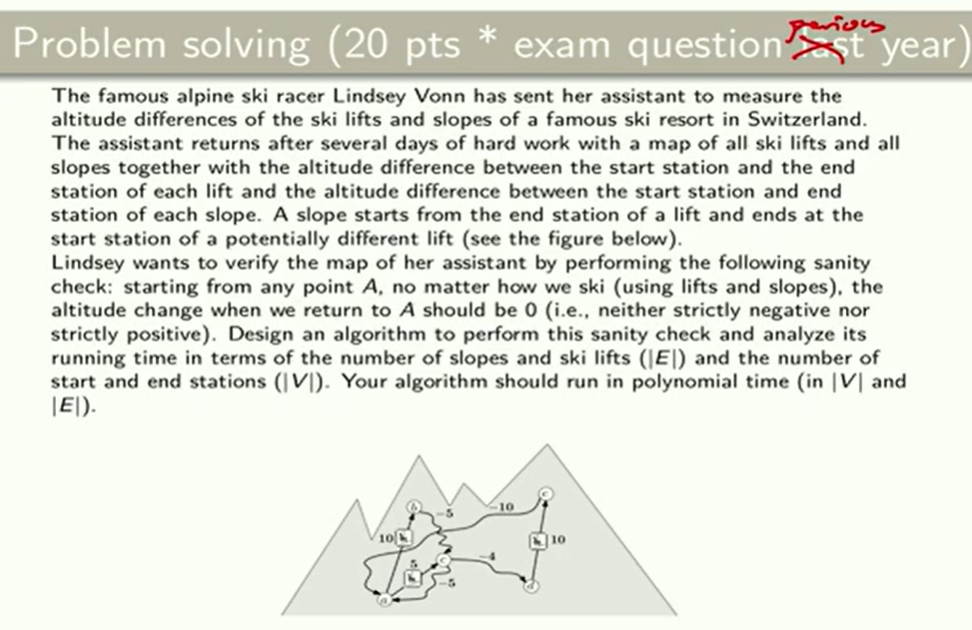
\includegraphics[width=\linewidth]{images/bellman-problem.png}
\end{exbox}

\paragraph{Idée.} La carte est cohérente si et seulement si tout cycle $C$ du graphe vérifie $W(C) = 0$. On décompose cette condition en deux :
\[
\forall C : W(C) = 0 \iff \bigl(\forall C : W(C) \geq 0\bigr) \;\textbf{ET}\; \bigl(\forall C : W(C) \leq 0\bigr)
\]
Chacune se vérifie avec Bellman-Ford en détectant l'absence de cycle négatif : une fois avec les poids $w$, une fois avec $-w$.

\paragraph{Pourquoi $|V|-1$ itérations suffisent.}
Un plus court chemin sans cycle a au plus $|V|-1$ arêtes. Après $|V|-1$ itérations de relaxation, toutes les distances correctes sont calculées.
\begin{itemize}
    \item \textbf{Pas de cycle négatif :} tout est stabilisé après $|V|-1$ itérations ; une $|V|$-ème ne relaxera plus rien.
    \item \textbf{Cycle négatif présent :} on peut indéfiniment réduire une distance en repassant par le cycle, donc la $|V|$-ème itération relaxe encore au moins une arête.
\end{itemize}

En exécutant Bellman-Ford deux fois (une fois avec $w$, une fois avec $-w$), la solution complète reste $O(|V| \cdot |E|)$.

\subsection{Dijkstra}

\begin{exbox}[title=Ce qu'il faut retenir]
\small\raggedright

\textbf{L'idée centrale.}
A chaque étape on finalise le sommet non-visité dont la distance
estimée est minimale. Cette distance est déjà optimale — car tous les poids sont
$\geq 0$, aucun chemin futur ne pourra la réduire.
C'est exactement ce qui distingue Dijkstra de Bellman-Ford : pas de deuxième chance,
pas de retour en arrière.

\textbf{Ce qui se passe à chaque itération.}
\begin{enumerate}
  \item On extrait $u = \arg\min_{v \in Q}\, v.d$ de la file.
  \item On l'ajoute à $S$ — sa distance est maintenant définitive.
  \item Pour chaque voisin $v$ de $u$ : si $u.d + w(u,v) < v.d$, on met à jour
        $v.d$ \emph{et} $v.\pi$.
\end{enumerate}

\textbf{Pourquoi ça ne marche pas avec des poids négatifs.}
Si une arête négative $(x, y)$ existe, un sommet $x$ déjà dans $S$ pourrait offrir un
chemin plus court vers $y$ mais $y$ est peut-être déjà finalisé.

\end{exbox}

\end{document}
